\documentclass[11pt,a4paper]{article}
\usepackage[hyperref]{acl2021}
\usepackage{times}
\usepackage{latexsym}
\renewcommand{\UrlFont}{\ttfamily\small}

\usepackage{subcaption}
\usepackage{microtype}
\usepackage{xcolor}
\usepackage{algorithm} 
\usepackage{amsmath}
\usepackage{algpseudocode}
\usepackage{graphicx}

\aclfinalcopy % Uncomment this line for the final submission
%\def\aclpaperid{***} %  Enter the acl Paper ID here

%\setlength\titlebox{5cm}
% You can expand the titlebox if you need extra space
% to show all the authors. Please do not make the titlebox
% smaller than 5cm (the original size); we will check this
% in the camera-ready version and ask you to change it back.

\newcommand\BibTeX{B\textsc{ib}\TeX}

\let\SUP\textsuperscript
\title{Per-node-depth GNN: using centrality measures to classify optimal depth}
%\author{$ \begin{matrix} \text{Rotem Ben Zion} \\ 211324975 \end{matrix} $\\[\bigskipamount]
%	rotm@campus.technion.ac.il}
%\author{Rotem Ben Zion,\quad Yonatan Belinkov,\quad Boaz Carmeli}
\author{$ \begin{matrix} \text{Rotem Ben Zion} \\ rotm@campus.technion.ac.il \end{matrix} \qquad \begin{matrix} \text{Niv Kook} \\ niv.ko@cs.technion.ac.il \end{matrix}$\\}

\date{June 2022}

\begin{document}
	
\maketitle
\begin{abstract}
Graph Neural Networks (GNNs) are neural networks designed to process data in graph form. Unlike other types of neural networks, empirical experiments show that the performance of GNNs drops significantly with large depths. Therefore, SOTA GNNs are shallow networks with few layers only.\\
In this project, we explore the idea of per-node-depth; the final representation of each node can be calculated by an individual amount of message-passing steps. More specifically, instead of a single classifier using the final (full-depth) representation, we train a node-classification network for each level of our GNN, and evaluate the optimal depth per node as a function of pre-calculated centrality measures. We analyze our results and deduct on the contribution of different node characteristics to its optimal depth.
\end{abstract}

\section{Introduction}
\label{sec:Introduction}
	Motivated by the success of Deep Learning (DL), several attempts have been made to apply DL models to non-Euclidean data; particularly, graph-structured data such as chemical compounds, social networks, and polygons. The idea of Graph Neural Networks (GNNs) was proposed in \cite{gori2005new} and \cite{scarselli2008graph}, which incited many research papers over the last two decades.\\
	one of the major problems in training GNNs is their struggle to propagate information between distant nodes in the graph \citep{alon2020bottleneck}. The distance between nodes is synonymous with the depth of the network, as the mechanism of GNNs operates by message-passing, which means the receptive field of a given node is simply the depth of the network in hop-distance. As a result, state-of-the-art GNN models are mostly shallow networks, in sharp contrast to the best performing models in other areas of DL such as Computer Vision and NLP. As will be discussed in section \ref{sec:RelatedWork} (related work), many papers presented potential causes, analysis and solutions to this phenomenon. However, most of these works implicitly assumed that depth should be constant over the graph, by inputting the final node embedding to a single trained classifier.\\
	In this project, we deviate from this convention, and apply per-node-depth; we insert a classifier after each message-passing layer, so that the node classification task can be done using different depths for different nodes. Our end goal is to investigate the question: \textbf{can the optimal depth of a given node be derived from its centrality measures in the graph?}\\
	To do so, we build a dataset by extracting centrality measures as features for each node, and assigning labels based on a comparison between the classifiers, as explained in section \ref{sec:OurMethod} and algorithm \ref{alg:OptimalDepth}. We then test the relationship between the features and labels in this new dataset by statistical analysis and by training ML models and testing their generalization and performance.
	Our hypothesis is that centrality measures should contain enough information to reasonably deduct the optimal depth. The justification for our hypothesis is that the well-established obstacle in GNN training - oversmoothing - directly relates to the amount of information aggregated by a single node, which in turn is intuitively correlated with the node's centrality.
	

\section{Related work}
\label{sec:RelatedWork}
	Many works in the past few years revolved around the exploration of depth in GNNs.\\
	The article "Do we need deep graph neural networks?" by Michael Bronstein \cite{towardsdatascience} discusses motivation for deep GNNs as well as possible explanations to the difference from networks in computer vision or NLP. \cite{oono2019graph} show the decrease in expressive power of GCNs (Graph Convolutional Network) as depth increases. \cite{alon2020bottleneck} propose an explanation to this phenomenon, claiming that GNNs are susceptible to a bottleneck when aggregating messages across a long path, causing \textit{over-squashing} of information. The authors in \cite{li2018deeper} suggest that the main difficulty in constructing deep networks is lying in over-smoothing. \cite{rong2019dropedge} attempt to deal with overfitting and over-smoothing by randomly dropping graph edges during each training epoch, and the authors of \cite{li2019deepgcns} use residual/dense connections and dilated convolutions to train a 56-layer GCN with good performance.
	More related to our project is the paper "RED-GCN: Revisit the Depth of Graph Convolutional Network", which suggests a method to find the optimal depth $d$ of a given graph without any prior knowledge and without the constraint to positive integers. However, the depth is still on a graph-level and not node-level. For the tasks of node classification and edge classification, the paper \cite{zeng2021decoupling} suggests a method which does allow individual depths, by first extracting localized subgraphs, and then applying GNNs with arbitrary depths on top of the subgraphs. Unfortunately, the extraction of subgraphs requires identifying the influential neighbors of each entity which is generally difficult.\\
	Lastly, on the topic of centrality measures, we consulted this \href{https://en.wikipedia.org/wiki/Centrality}{Wikipedia page}.

\section{Our method}
\label{sec:OurMethod}
	As previously mentioned, our goal is to test whether node centrality measures contain sufficient information to determine the optimal depth of a given node. This entails a few challenges:
	\begin{itemize}
		\item How can we evaluate, over the nodes in our training set, which depth is optimal?
		\item How can we capture the relationship between the extracted features and the optimal depth?
	\end{itemize}
	With these challenges in mind, we propose the following method. Let $max\_depth$ be the upper bound on depths we wish to test. The method consists of three main steps.
	\begin{enumerate}
		\item We define a GCN with $max\_depth$ message-passing layers. We insert a classifier after each layer, denoted by $\{clf^{(i)}\}_{i=1}^{max\_depth}$. The loss used to train the network will now be the simple summation of losses. The training procedure is specified in alorithm \ref{alg:NetworkTrainProcedure}.
		\item After the network and classifiers are trained, we take a new set of heldout nodes, and for each we compare the different classifiers and extract the best one (loss-wise). This will be defined as the label in our new dataset. Pseudocode for this process presented in algorithm \ref{alg:OptimalDepth}.
		\item We use our newly created dataset to train a classification model. The model choice is done via cross-validation and can be a decision tree or an MLP. We then use the fitted classifier to test generalization and the influence of different centrality measures as desired.
	\end{enumerate}

	\subsection*{Centrality measures}
		In this subsection, we list the centrality measures used in our implementation.
		\begin{enumerate}
			\item \textbf{in-degree}: number of edges into the node.
			\item \textbf{out-degree}: number of edges out of the node.
			\item \textbf{PageRank}: importance estimatation by counting the number and quality of edges into the node.
			\item \textbf{Hubs}: part of the HITS algorithm, measures how well the node points to good authorities.
			\item \textbf{Authorities}: part of the HITS algorithm, measures how many good hubs point to the node.
			\item \textbf{Katz centrality}: computes the relative influence of a node, by counting neighbors of different hop distances with a discount factor.
			\item \textbf{Perculation}: attempts to evaluate how "infectious" the node is, by counting the proportion of shotest paths that go through the node.
			\item \textbf{Eigenvector centrality}: assigns a relative score based on the concept that connections to high-scoring nodes contribute more than equal connections to low-scoring nodes. PageRank and Katz centrality are variants of the eigenvector centrality.
		\end{enumerate}
	Imortant note: several centrality measures were numerically impossible to compute, time-wise or memory-wise. For example, the betweenness measure. This could potentially be solved by calculating the measures on subgraphs, but as this project's goal is a proof of concept, we have decided to only use the centrality measures stated above.
	
	\begin{algorithm*}
		\caption{Network Training Procedure}
		\label{alg:NetworkTrainProcedure}
		\begin{algorithmic}[1]
			\For {batch in Training Set}
			\State $X = \text{batch.features}$
			\State $y = \text{batch.labels}$
			\State $\text{loss}=0$
			\For {$i \in \{1,2,\dots,\text{max\_depth}\}$}
			\State $X = layer^{(i)}(X)$
			\State $\text{pred} = clf^{(i)}(X)$
			\State $\text{loss} = \text{loss} + \text{cross\_entropy}(\text{pred}, y)$
			\EndFor
			\State $W_{\text{network}} = W_{\text{network}} - \alpha \cdot \nabla \text{loss}$
			\EndFor
		\end{algorithmic} 
	\end{algorithm*}

	\begin{algorithm*}
	\caption{Optimal-depth Data Creation}
	\label{alg:OptimalDepth}
	\begin{algorithmic}[1]
		\State Assume $\{layer^{(i)}\}_{i=1}^{\text{max\_depth}}, \{clf^{(i)}\}_{i=1}^{\text{max\_depth}}$ are trained on the training set
		\State Initialize an empty dataset $D = \emptyset$
		\For {node in a heldout dataset}
		\State $X = \text{node.features}$
		\State $y = \text{node.label}$
		\State $\text{clf\_scores} = \{\}$
		\For {$i \in \{1,2,\dots,\text{max\_depth}\}$}
		\State $X = layer^{(i)}(X)$
		\State $\text{pred} = clf^{(i)}(X)$
		\State $\text{clf\_scores}[i] = \text{cross\_entropy}(\text{pred}, y)$
		\EndFor
		\State $\text{depth\_label} = \arg \min \text{clf\_scores}$
		\State $\text{centrality\_features} = \text{precalculated\_cent\_features}(\text{node})$
		\State Add data point $(\text{centrality\_features}, \text{depth\_label})$ to $D$
		\EndFor
		\State Return $D$
	\end{algorithmic} 
\end{algorithm*}


\section{Experiments}
\label{sec:Experiments}
	In order to test our hypothesis, we have implemented the following set of experiments.
	\begin{itemize}
		\item Optimal depth histogram, to cehck class imbalance in our new dataset
		\item Performance and generalization of the depth classifier with different max\_depth values
		\item Correlation heatmap of the different centrality measures with the optimal depth
	\end{itemize}
	The dataset used in our implementation is the obgn-arxiv dataset \citep{hu2020open}.\\
	All code, including network training, depth classifier, data processing and experiments is available on \href{https://github.com/Rotem-BZ/GeometricDL_project}{GitHub}. All of the experiments were run on Intel(R) Core(TM) i7-8565U CPU @ 1.80GHz (personal computer).
	
\section{Results}
\label{sec:Results}
	\subsubsection*{Distribution of Optimal Depth}
	In figure \ref{fig:histogram}, we present histograms for the label distribution in our new dataset, i.e., how many nodes correspond to each optimal depth. Note that when training the depth classifier, we use under-sampling to counter the class imbalance. There is a visible change in distribution between the train and heldout node sets. One possible explanation to this difference is a distribution shift between the nodes, caused by the temporal data split used to create them (the train set consists of papers published earlier). This leads to unexpected performance in the data creation process over the heldout set.

	\begin{figure}[t!]
		\centering
		\begin{subfigure}[t]{0.25\textwidth}
			\centering
			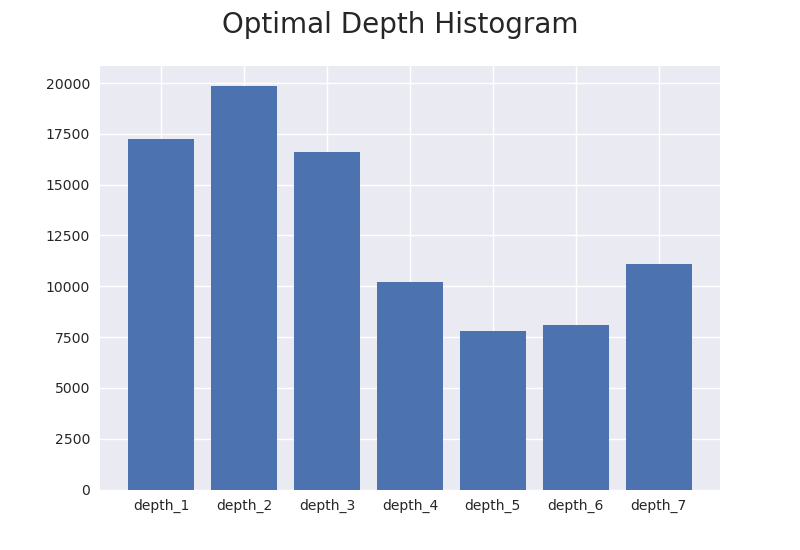
\includegraphics[width=1\linewidth]{images/optimal_depth_histogram_train.png}
			\caption{train set}
		\end{subfigure}%
		~ 
		\begin{subfigure}[t]{0.25\textwidth}
			\centering
			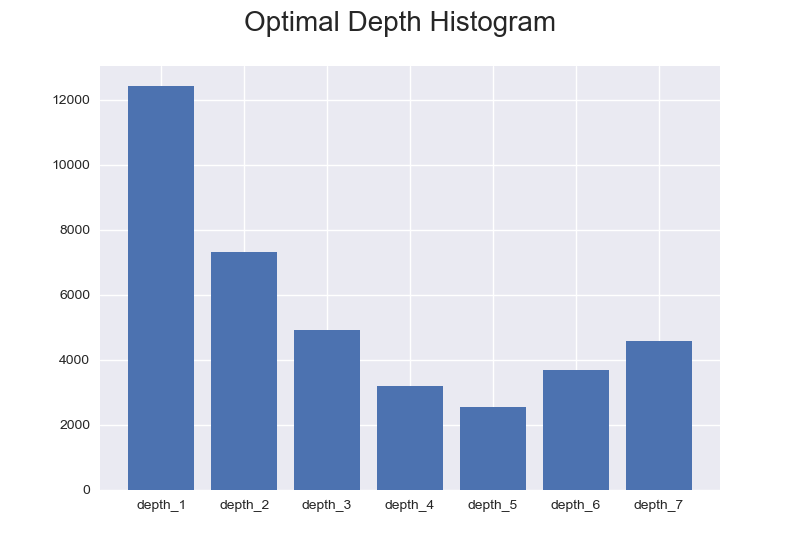
\includegraphics[width=1\linewidth]{images/optimal_depth_histogram.png}
			\caption{heldout set}
		\end{subfigure}
		\caption{Histograms of optimal depths}
		\label{fig:histogram}
	\end{figure}


	\subsubsection*{Performance and Generalization of the Depth Classifier}
	For this experiment, let GNN-train, GNN-validation and GNN-test be the subgroups of nodes used to train the original network. We performed the data creation procedure (algorithm \ref{alg:OptimalDepth}) to create three matching datasets, so that GNN-test is the heldout set of nodes used in the other experiments.\\
	For each dataset and for each max\_depth in $\{3, 5, 7\}$, we compared different ML models via cross-validation. Table \ref{tab:clf_performance} shows the best model and its accuracy per max\_depth. The accuracy is calculated over a test dataset.\\
	While all models improved upon the random baseline, none improved by a significant margin; the objective classification accuracy is low. This contradicts our hypothesis, and will be discussed in section \ref{sec:Discussion}. The effect of the source dataset for data creation models the effect of distribution shift, and we can clearly see that the GNN-test generated dataset leads to worse performance compared to GNN-train. In addition, GNN-test always prefers the AdaBoost model while GNN-train leads to similar results for the different models. There is no clear relationship between max\_depth and the best ML model.\\
	Following the results in table \ref{tab:clf_performance}, we considered adding the node's initial features to the centrality features before classification. The corresponding results are shown in table \ref{tab:clf_performance_combined}. The accuracy when training and evaluating on the GNN-test dataset improved marginally, but results on GNN-train decreased. The general trend hasn't changed.
	\begin{table*}[t]
		\centering
		\begin{tabular}{c|cccc}
			\hline
			\textbf{max\_depth} & \textbf{GNN-train} & \textbf{GNN-validation} & \textbf{GNN-test} & \textbf{random model} \\
			\hline
			3 & B, 35.31 & B, 36.6 & B, 34.88 & 33.3 \\
			5 & D, 23.04 & C, 21.55 & B, 21.58 & 20.0 \\
			7 & C, 17.15 & B, 18.29 & B, 16.82 & 14.29 \\\hline
		\end{tabular}
		\caption{best model and accuracy (\%) over different sets and max\_depths. Model index: (A) - decision tree, (B) - AdaBoost, (C) - Random Forest, (D) - MLP}\label{tab:clf_performance}
	\end{table*}

	\begin{table*}[t]
		\centering
		\begin{tabular}{c|cccc}
			\hline
			\textbf{max\_depth} & \textbf{GNN-train} & \textbf{GNN-validation} & \textbf{GNN-test} & \textbf{random model} \\
			\hline
			3 & 32.95 & 36.53 & 37.06 & 33.3 \\
			5 & 19.98 & 23.14 & 21.77 & 20.0 \\
			7 & 14.35 & 17.10 & 17.14 & 14.29 \\\hline
		\end{tabular}
		\caption{best model and accuracy (\%) over different sets and max\_depths, trained and evaluated with centrality features as well as the graph features used for node classification. The model used is AdaBoost.}\label{tab:clf_performance_combined}
	\end{table*}

	\subsubsection*{Correlation heatmap}
	Figure \ref{fig:correlation_heatmap} shows a correlation heatmap including the centrality measures and optimal depth labels. The bottom line (or right column) contains correlations of the features with the label, and we see little to no correlation. This result is in par with the poor performance of the depth classifiers we have seen in the previous experiment. Some possible explanations are discussed in the next section.
	\begin{figure}[h]
		\centering
		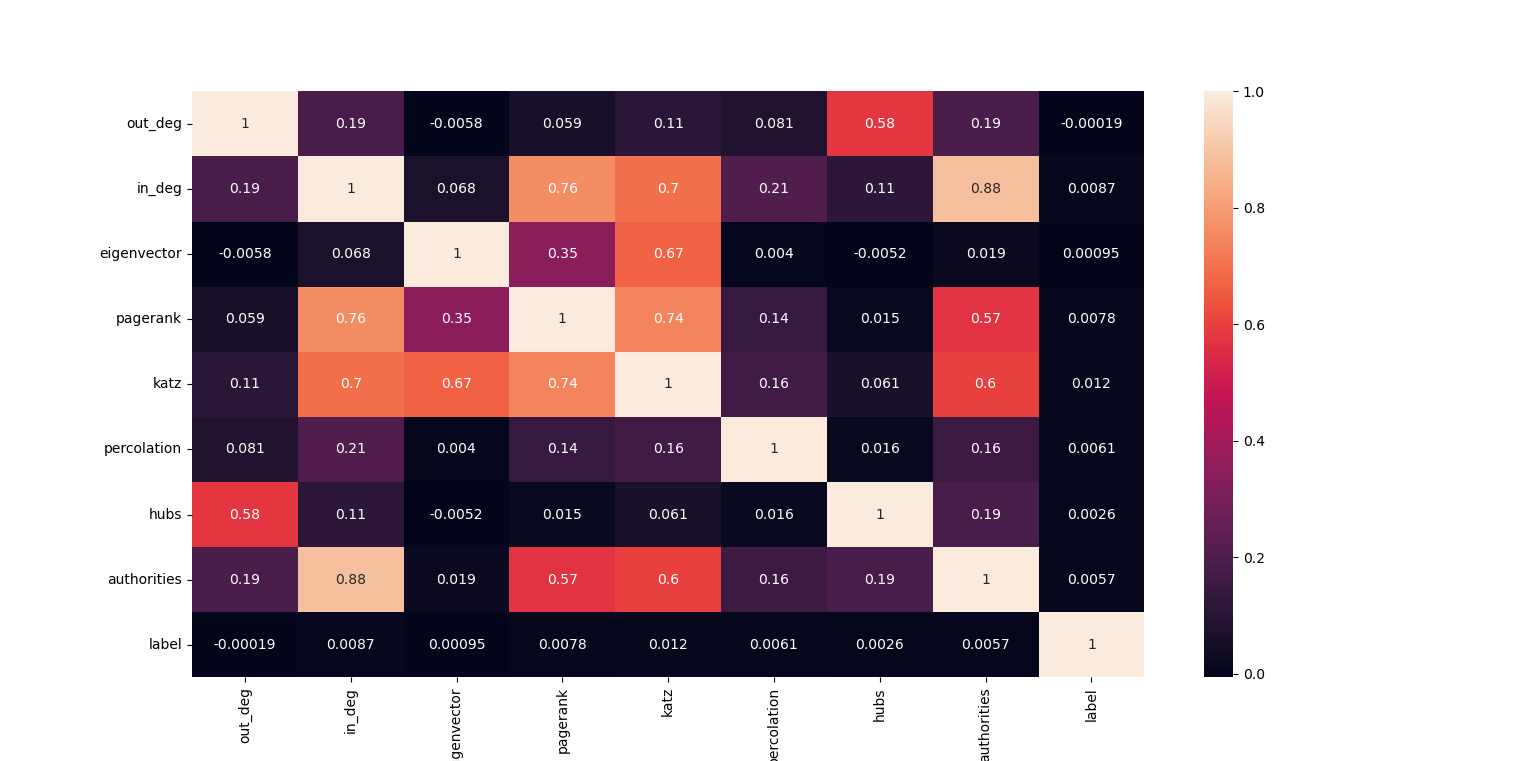
\includegraphics[width=1\linewidth]{images/correlation_heatmap_depth5_testset.png}
		\caption{Correlation heatmap for centrality features and optimal depth}
		\label{fig:correlation_heatmap}
	\end{figure}

\section{Discussion}
\label{sec:Discussion}
In our experiments, specifically the depth classifier's performance and the correlation heatmap, we encountered surprising results; the ML models were not able to generalize well despite a reasonable amount of data (minimum of 30,000 data points in GNN-validation before train-test split), and the correlation between the centrality features to the label is non-existent. These results suggest the opposite from our hypothesis - that the centrality measures do not contain sufficient information to classify optimal depth. However, several other explanations are possible:
\begin{itemize}
	\item Our GNN training procedure (algorithm \ref{alg:NetworkTrainProcedure}) is not optimal. For example, the first message-passing layer is optimized by the loss from every classifier in every trining batch, while the last layer is only optimized by loss generated from the last classifier. We used SAGEconv layers with batch normalization, and possibly could have tweaked parameters better. In the extreme case of 7 layers, the minimal train loss is 1.0, and minimal test loss is 1.45. For comparison, a random model generates loss of 3.6.
	\item Temporal data split. Distribution shift may cause unpredictable labels in our created dataset.
	\item Limitation of centrality measures. Many informative centrality measures can't be efficiently computed over large graphs, such as betweenness and closeness. Extracting additional features may improve the results.
\end{itemize}
In retrospect, there are several arguments supporting the null hypothesis:
\begin{itemize}
	\item Predicting the optimal depth may be even more difficult than solving the node classification problem. Thus, it will not be a simple function of centrality measures.
	\item The performance of the classifiers should intuitively depend on the embedding of nodes throughout the network's forward pass, which encapsulates their centrality features via message-passing. However, it may include important additional information, and therefore using only centrality is not enough to classify optimal depth.
\end{itemize}

\pagebreak
\section{Summary and future work}
\label{sec:SummaryFuture}
In this project, we have implemented a GNN training procedure which allowes node classification to be accomplished with a different number of message-passing steps per node. We used this idea to create a new dataset, in which the labels are the layer indices in which node classification loss is minimal. We attempted to find a connection between said labels and a set of 8 precalculated centrality measures of each node, by correlation and by training ML models for classification. We haven't found any reliable connection and deducted that additional information or stronger models are required to do so. Future work may investigate the following questions:
\begin{itemize}
	\item Can we find a connection between optimal depth and the hidden node embeddings throughout the network's forward pass?
	\item Will similar results be found on other graph datasets?
	\item What is the effect of homophilic vs heterophilic input graph on the correctness of our hypothesis?
	\item What is the effect of the input graph's size on the correctness of our hypothesis?
	\item Can per-node-depth be succesfully applied to DL methods in other areas? such as Convolutional Neural Networks in Computer Vision tasks?
\end{itemize}


\bibliographystyle{acl_natbib}
\bibliography{references}


\end{document}
